\documentclass[a4paper,12pt]{article}   % papír A4, písmo 12 bodu
\usepackage[utf8x]{inputenc}            %kodovaní UTF-8
\usepackage{ucs}                        %kodovani unicode
\usepackage[czech]{babel}               %podpora cestiny
\usepackage[T1]{fontenc}                %pouzij variantu pisma T1 (hacky, carky)
\usepackage[left=2.5cm,right=1.5cm,top=2.5cm,bottom=2.5cm]{geometry} %okraje stranky
\usepackage{amsmath,amsfonts,amssymb}   %podpora matematiky
\usepackage{gensymb,marvosym}           %symboly celsius (\celsius) apod.
%\usepackage{mathptmx}                   %font Times New Roman s~podporou matematiky
\usepackage{times}                      %font Times New Roman (matematika pismem Computer Modern) 
\usepackage{parskip}                    %mezera mezi odstavci
%\usepackage[document]{ragged2e}         %text zarovany vlevo
\usepackage[none]{hyphenat} \sloppy     %slova nedelit a~nepretekat
\usepackage{titlesec}
\setcounter{secnumdepth}{4}
\clubpenalty 10000                      %kontrolovat sirotky
\widowpenalty 10000                     %kontrolovat vdovy
\usepackage{setspace} \onehalfspacing   %podpora pro zmenu radkovani + radkovani 1,5
\usepackage{enumerate}                  %podpora pro zmenu cislovani
\usepackage{fancyhdr}                   %vlastni zahlavi a~zapati
\usepackage{graphicx}                   %podpora grafiky
\graphicspath{{materialy/}}             %vychozi adresar s~obrazky
\usepackage{caption}                    %popisky
\usepackage{subcaption}                 %podpopisky
\usepackage{siunitx}
\usepackage{MnSymbol,wasysym}
\usepackage[shortlabels]{enumitem}
\usepackage{amsmath}
\usepackage{lastpage}                   %zjištění poslední stránky \pageref{LastPage}
\usepackage{float}                      
\usepackage{url}
\usepackage[unicode]{hyperref}          %klikaci odkazy v~textu
\usepackage{mhchem}
\usepackage{multirow}

\usepackage{halloweenmath}


\titleclass{\subsubsubsection}{straight}[\subsection]
\newcounter{subsubsubsection}[subsubsection]
\renewcommand\thesubsubsubsection{\thesubsubsection.\arabic{subsubsubsection}}
\renewcommand\theparagraph{\thesubsubsubsection.\arabic{paragraph}} % optional, useful if paragraphs are to be numbered


%------------------------ čtvrtá a~pátá úroveň nadpisu ---------------------------

\titleformat{\subsubsubsection}
  {\normalfont\normalsize\bfseries}{\thesubsubsubsection}{1em}{}
\titlespacing*{\subsubsubsection}
{0pt}{3.25ex plus 1ex minus .2ex}{1.5ex plus .2ex}

\makeatletter

\renewcommand\paragraph{\@startsection{paragraph}{5}{\z@}%
  {3.25ex \@plus1ex \@minus.2ex}%
  {-1em}%
  {\normalfont\normalsize\bfseries}}
\renewcommand\subparagraph{\@startsection{subparagraph}{6}{\parindent}%
  {3.25ex \@plus1ex \@minus .2ex}%
  {-1em}%
  {\normalfont\normalsize\bfseries}}
\def\toclevel@subsubsubsection{4}
\def\toclevel@paragraph{5}
\def\toclevel@paragraph{6}
\def\l@subsubsubsection{\@dottedtocline{4}{7em}{4em}}
\def\l@paragraph{\@dottedtocline{5}{10em}{5em}}
\def\l@subparagraph{\@dottedtocline{6}{14em}{6em}}
\makeatother

\setcounter{secnumdepth}{4}
\setcounter{tocdepth}{4}


\setlist[enumerate]{itemsep=0mm}
%_____________________________|___________________________|_____________________________%
%                             |                           |                             %
%-----------------------------| ZDE VYPLNIT UDAJE O PRACI |-----------------------------%
%_____________________________|___________________________|_____________________________%
%                             

\newcommand{\nazev}{Demonstrace principu vzorkování}                                                        %
\newcommand{\jmeno}{Jakub Dvořák}                                                     %
\newcommand{\datum}{12.11.2020}                                                              %
%---------------------------------------------------------------------------------------%


%-----------------------------| POUŽITÁ MAKRA |-----------------------------%

%\newcommand{\zkratka}{ve výsledku se mi napíše tenhle text}
%\newcommand{}{}
%\newcommand{}{}
%\newcommand{}{}
\newcommand{\tsub}[1]{$_\textrm{#1}$}
\newcommand{\texp}[1]{$^\textrm{#1}$}
\newcommand{\tohm}{$\Omega$}
\newcommand{\tmu}{$\mu$}
\newcommand{\tpm}{$\pm$}



%_______________________________________________________________________________________%
%_______________________________________________________________________________________%


%----------------------------------- KONEC PREAMBULE -----------------------------------%






%-------------------------------------- DOKUMENT --------------------------------------%
%______________________________________________________________________________________%
\begin{document} %%%%%%%%%%%%%%%%%%%%%%%%%%%%%%%%%%%%%%%%%%%%%%%%%%%%%%%%%%%%%%%%%%%%%%%

\setcounter{page}{0} %cislo strany
\pagestyle{empty} %stranku necislovat

%prostredi pro grafy a~schemata \begin{graf} \begin{schema}
\newfloat{schema}{htbp}{schema}\floatname{schema}{Schéma}
\newfloat{graf}{htbp}{graf}\floatname{graf}{Graf}

\begin{titlepage}
    \begin{center}
        \vspace*{1cm}
            
        \Huge
        \textbf{\nazev}
            
        \vspace{0.5cm}
        \LARGE
            
        \vspace{1.5cm}
            
        \textbf{\jmeno}
            
        \vfill
            
        \vspace{0.8cm}
            
        \Large
            
        \datum\\
        \vspace*{.5cm}
        
\includegraphics[width=.4\textwidth]{logo-cvut-fee.png}\\
    \end{center}
\end{titlepage}

% --- definice zapati a~cislovani ---
\newpage 
\pagestyle{fancy}                                       %vlastni zahlavi/zapati
\renewcommand{\headrulewidth}{0pt}                      %bez linky v~zahlavi
\renewcommand{\footrulewidth}{.5pt}                    %linka v~zapati - optional
\lhead{}       \chead{} \rhead{\nazev}                        %pole zahlavi (prazdna)
\lfoot{\jmeno} \cfoot{} \rfoot{\thepage}   %pole zapati


%------------------------------------ VLASTNÍ TEXT ------------------------------------%



\section{Úkol měření}
\label{chap:ukol}
\begin{enumerate}
    \item Pomocí přípravku se vzorkovačem, jehož blokové schéma je nakresleno na obr. \ref{fig:zapojeni}, zobrazte na osciloskopu ovzorkovaný průběh harmonického napětí z generátoru s~frekvencí v~rozmezí 200 až 1100~Hz a~efektivní hodnotou 1 až 3~V.
    \item V režimu "ruční vzorkování" sledujte na číslicovém voltmetru změnu hodnoty ovzorkovaného výstupního napětí $U_{výst}$ v~závislosti na čase (chyba v~režimu pamatování), stanovte velikost této změny za 10~s a~přepočtěte ji na mV/ms.
    \item S použitím časové lupy na osciloskopu zkontrolujte průběh napětí $U_{výst}$ na výstupu v~časovém intervalu "upnutí" – viz. monografie Haasz, V., Sedláček, M.: \textit{Elektrická měření. Přístroje a~metody}, kap. 4 - a~určete přibližně upínací dobu.
    \item V režimu přípravku "1 ze 16" změřte pomocí stejnosměrného číslicového voltmetru postupně všech 16 hodnot vzorků napětí, časový průběh signálu graficky rekonstruujte, vypočtěte efektivní hodnotu rekonstruovaného signálu a~porovnejte výsledek s hodnotou změřenou střídavým číslicovým voltmetrem přímo na funkčním výstupu generátoru.
    
\end{enumerate}
%pro subseznam ->
%\item \begin{enumerate}[label=\alph*)]
%  \item 
%\end{enumerate}

\section{Schéma zapojení}
\label{chap:schema_zapojeni}
\begin{figure}[h!]
  \centering
  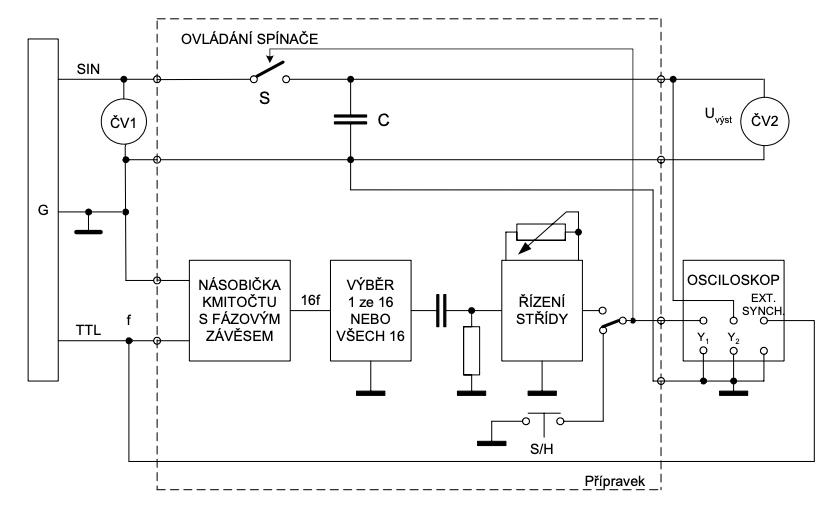
\includegraphics[width=.6\textwidth]{schema_zapojeni.png}
  \caption{Zapojení přípravku pro demonstraci principu vzorkování}
  \label{fig:zapojeni}
\end{figure}


\section{Seznam použitých přístrojů}
\label{chap:seznam_pristroju}
\begin{table}[H]
  \begin{tabular}{ll}
        G & generátor funkcí Instek GFG-8020H\\
        ČV1 & číslicový multimetr GDM-8145, rozsah 2~V, přesnost \tpm (0,03 \% z údaje + 4 digity)\\
        ČV2 & číslicový multimetr DM-441B, rozsah 2~V, přesnost \tpm (0,01 \% z údaje + 4 digity)\\
        OSC & osciloskop Keysight DSOX2002A, 5~\tmu S/div\\
  \end{tabular}
\end{table}

\section{Teoretický úvod}
\label{chap:teoreticky_uvod}
Při měření harmonických průběhu pracujeme se spojitými jevy, jako ostatně všude v~našem světě. Při měření digitálními přístroji nicméně potřebujeme získat diskrétní data a~tedy spojitý signál rozkouskovat. K tomuto nám slouží vzorkovač. Ten v~předem definovaných intervalech změří měřenou veličinu a~její hodnotu poté po dobu intervalu sledování drží, abychom ji mohli odečíst. Při příliš malém vzorkování může docházet k chybnému měření. To je způsobeno změnou veličiny za dobu, kterou vzorkovač drží dříve změřenou hodnotu.

\section{Naměřené hodnoty}
\label{chap:namerene_hodnoty}
V tabulkách níže jsou zaznamenány z jednotlivých měření.
\begin{table}[h!]
  \centering
  \begin{tabular}{|c|c|}
    \hline
    $f$ [Hz]&$U_{ef}$ [V]\\\hline\hline
    500&1,5839\\\hline
  \end{tabular}
  \caption{Naměřené napětí}
  \label{tab:napeti}  
\end{table}

\begin{table}[h!]
  \centering  
  \begin{tabular}{|l|c|}
    \hline
    čas [s]&Napětí [V]\\\hline\hline
    1&2,09  \\\hline
    2&2,075 \\\hline
    3&2,059 \\\hline
    4&2,043 \\\hline
    5&2,028 \\\hline
    6&2,013 \\\hline
    7&1,998 \\\hline
    8&1,983 \\\hline
    9&1,969 \\\hline
    10&1,954 \\\hline
  \end{tabular}
  \caption{Závislost hodnoty sledovaného napětí na čase}
  \label{tab:sledovane}  
\end{table}

\begin{table}[h!]
  \centering
  \begin{tabular}{|l|c|}
    \hline
    Vzorek $n$&Napětí [V] \\\hline\hline
    1&1,704\\\hline
    2&0,925\\\hline
    3&0,058\\\hline
    4&-0,764\\\hline
    5&-1,423\\\hline
    6&-1,82\\\hline
    7&-1,911\\\hline
    8&-1,621\\\hline
    9&-1,063\\\hline
    10&-0,292\\\hline
    11&0,572\\\hline
    12&1,404\\\hline
    13&2,07\\\hline
    14&2,477\\\hline
    15&2,571\\\hline
  \end{tabular}
  \caption{Hodnota napětí jednotlivých vzorků}
  \label{tab:vzorky}  
\end{table}



\section{Zpracování naměřených hodnot}
\label{chap:zpracovani_hodnot}
Podle tabulky \ref{tab:sledovane} je pokles napětí za 10~s roven 0,136~V. To odpovídá hodnotě 0,0136~V/s resp. 0,0136~mV/ms.

Velikost časového intervalu upnutí byl odečten z osciloskopu jako 2,5~\tmu s.

Zrekonstruovaný graf naměřených napětí vzorků je zobrazen v~grafu \ref{graf:vzorky}.

\begin{graf}
  \centering
  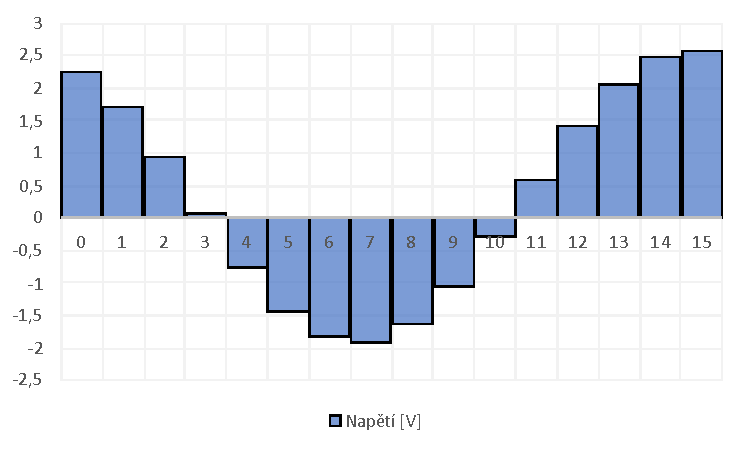
\includegraphics[width=.8\textwidth]{graf_vzorky.pdf}
  \caption{Velikosti napětí jednotlivých vzorků, data z tabulky \ref{tab:vzorky}}
  \label{graf:vzorky}
\end{graf}.

Pro výpočet efektivní hodnoty u průběhu napětí, tvořeného obdélníkovými průběhy nám stačí spočítat plochu pod grafem. K tomu využijeme následující vrozec.
\begin{equation}
  U_{ef} = \sum_{n=0}^{15} \frac{|\,U_n\,|}{16}
\end{equation}
Hodnota efektivního napětí $U_{ef}$ poté vyjde 1,43~V. Relativní chyba oproti hodnotě naměřené číslicovým multimetrem je 0,09 resp. 9~\%.


\section{Závěrečné vyhodnocení}
\label{chap:zaver}
Zjistili jsme, že při použití vzorkování dochází hned k několika chybám měření. Pokud je doba pamatování příliš dlouhá, začne držené napětí klesat. To je způsobeno vybíjením nabitého kondenzátoru, který je nabit na hodnotu odpovídající zobrazenému napětí. Toto jde zvýšit větší kapacitou kondenzátoru, nebo kvalitnějším operačním zesilovačem.

Další chyba vznesená do měření je způsobena držením hodnot, ačkoliv se měřená hodnota stále mění. Tato chyba ale není tak zásadní, jak by se na první pohled zdálo, jelikož plocha grafu, která v~grafu přebývá držením hodnot napětí je stejná jako plocha grafu, která chybí.



%--- LITERATURA a~ZDROJE (povinne) ---
\clearpage
\renewcommand{\refname}{Seznam použité literatury a~zdrojů informací} 
%\section*{Seznam použité literatury a~zdrojů informací}
\phantomsection %pridej odkaz do PDF zalozek
\addcontentsline{toc}{section}{Seznam použité literatury a~zdrojů informací}

\begin{thebibliography}{99}

%----------------------------------------------------
\subsection*{Seznam použitých internetových zdrojů}
    \bibitem{navod} Návod k~laboratorní úloze
    
\end{thebibliography}

\end{document}